\chapter{Simulation Framework}
The methods described in Chapter \ref{ch:pp} on Path Planning were implemented within a simulation environment in \textit{MATLAB} in order to show the effectiveness of the introduced path planners. The target fields in the simulations are represented as randomly generated matrices of a desired size. The autocorrelation factor of the field in the simulation is an adjustable factor that determines the likeliness of each pair of neighboring points as a function of distance. 

For a given waypoint destination, a simulated vehicle will pass over every vesicle on the line connecting its original position and its final position. The vehicle's heading angle can be controlled at any point in the simulation. The path planner directly feeds a control heading angle to the simulated vehicle. A trajectory (a set of waypoints), $T$, calculated in Chapter \ref{ch:pp}, is loaded into a waypoint queue for the vehicle, where each waypoint is met one after another. After meeting the final waypoint in the trajectory, the next set of waypoints is calculated by a path planner. The process continues until the termination condition (maximum area scanned) is satisfied. A sample is taken at every possible vesicle that the vehicle passes over. The location and value of each sample is stored in the vehicle object's memory for later use in the prediction procedures.

\section{Generating a Target Field}
The simulation yields a target field that is of variable height $h$, and width $w$. Each vesicle in the field is exactly the area of the sensor footprint of the simulated vehicle's sensor. This is to make the sensor measurements as ideal as possible, so no samples are missed when a vesicle is scanned.

The field is composed of a single feature which is autocorrelated spatially. Initially, the points on the field are generated from a normal distribution with a standard deviation of $1$, and expected value of $0$. The field is then convolved with a two dimensional Gaussian filter, $G(x,y,\sigma_{field})$ (Equation \ref{eq:gauss_filt}), with a variable standard deviation, $\sigma_{field} \in \mathbb{R}_{\geq 0}$ which sets the radius of the filter. 

\begin{equation}
G(x,y,\sigma_{field}) = \frac{1}{2 \pi \sigma_{field}^2} e^{\frac{x^2 + y^2}{2\sigma_{field}^2}}
\label{eq:gauss_filt}
\end{equation}

\noindent where $x \in \mathbb{N}$, $y \in \mathbb{N}$, and for all values $x \in [1, w], y \in [1, h]$.

The Gaussian filter ``smooths'' the field in order to simulate autocorrelation. In \textit{MATLAB}, the \textit{imfilter} function is used to perform a 2D convolution on the randomly generated field. The result is a randomly-generated, variably-sized, and autocorrelated field with a unit-less feature of interest. One such field can be observed in Figure \ref{fig:gen_field}. As the value of the standard deviation of the Gaussian filter kernel, $\sigma_{field}$, increases, the field exhibits higher spatial autocorrelation. Inversely, when $\sigma_{field}$ is close to zero, the field becomes has no signs of spatial autocorrelation.

% \begin{figure}[htb!]
% 	\begin{subfigure}
% 		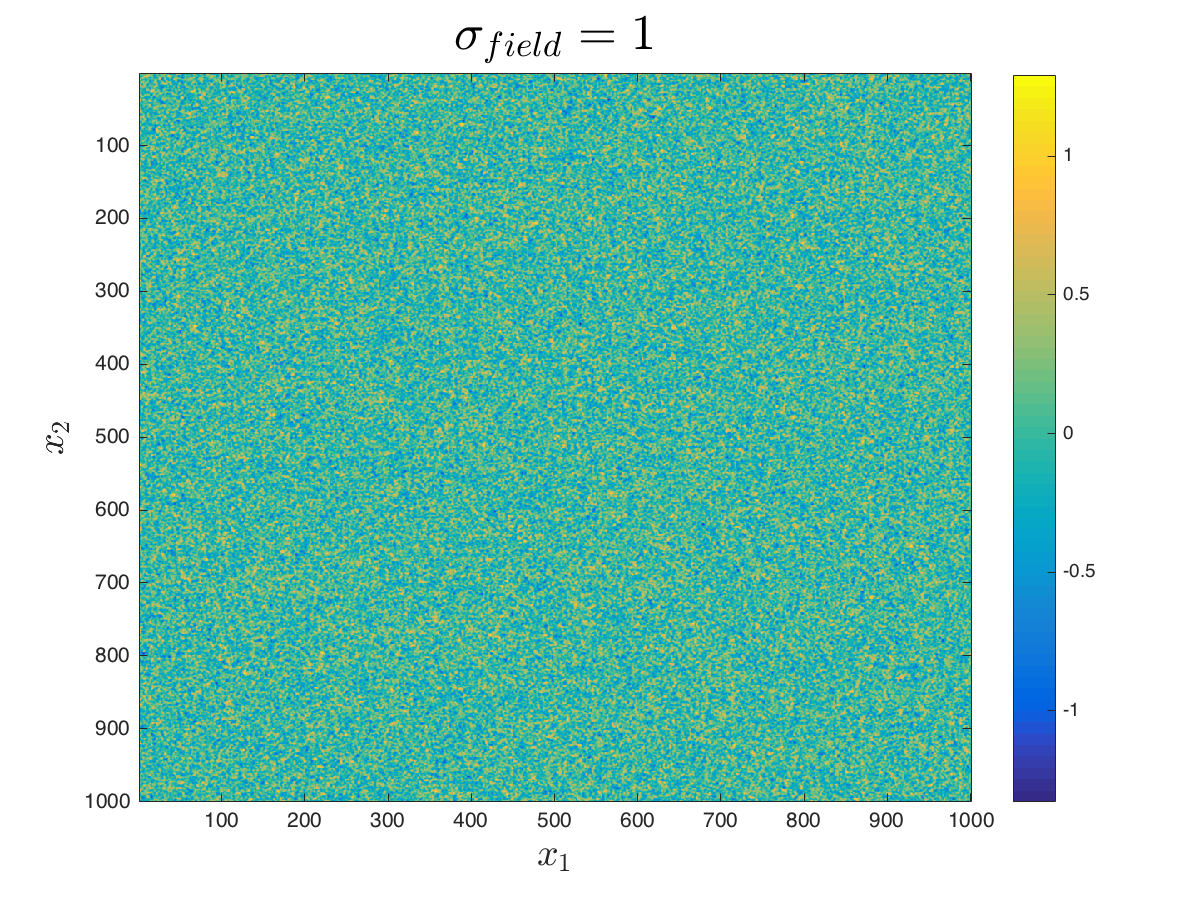
\includegraphics[width=0.45\linewidth]{figures/autocorr_sigma_1.png}
% 		\subcaption{$\sigma_{\text{field}} = 1$. The field apears to exhibit very low spatial autocorrelation.}
% 	\end{subfigure}
% 	~
% 	\begin{subfigure}
% 		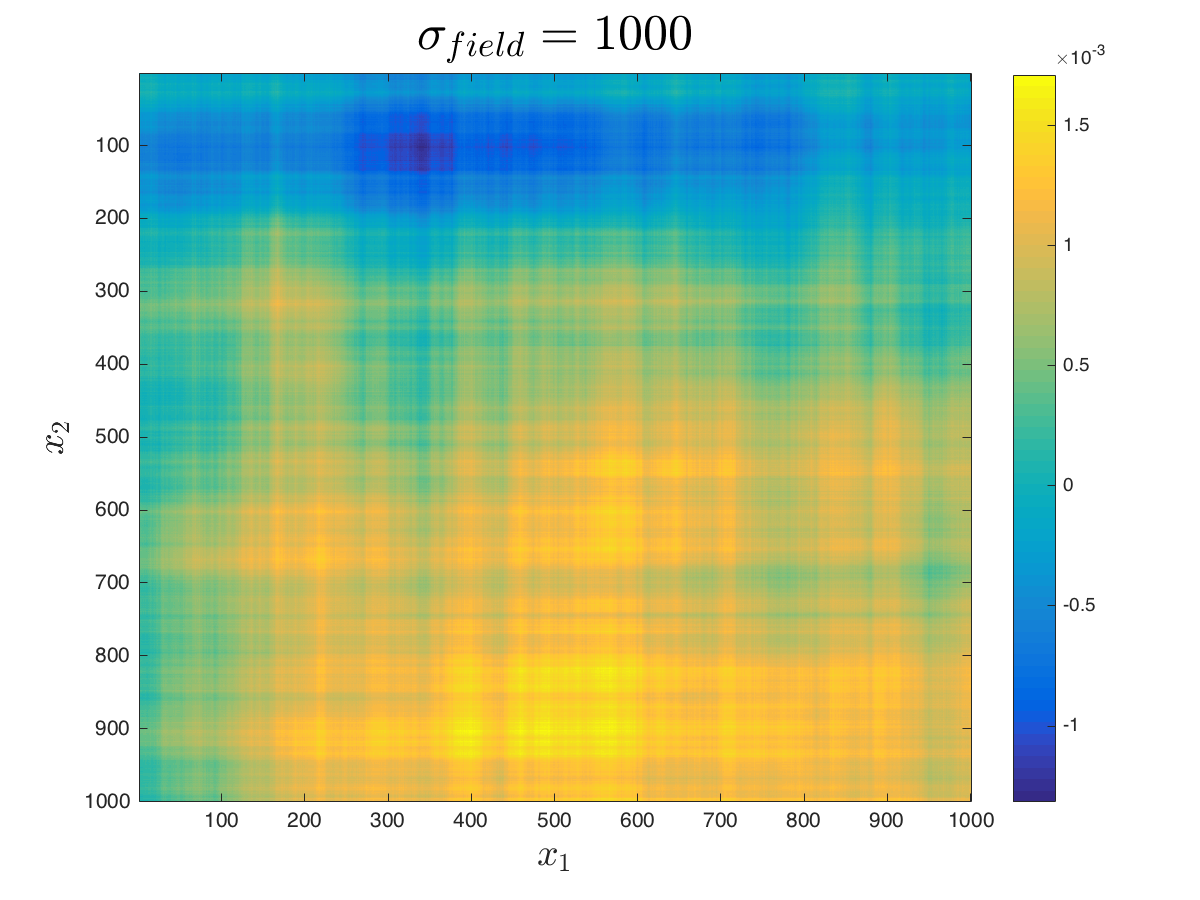
\includegraphics[width=0.45\linewidth]{figures/autocorr_sigma_1000.png}
% 		\subcaption{$\sigma_{\text{field}} = w$, where $w = 1000$ is the field width and height. The field is more spatially autocorrelated.}
% 	\end{subfigure}
% \end{figure}

\begin{figure}[ht!]
    \centering
    \begin{subfigure}[t]{0.33333\textwidth}
        \centering
        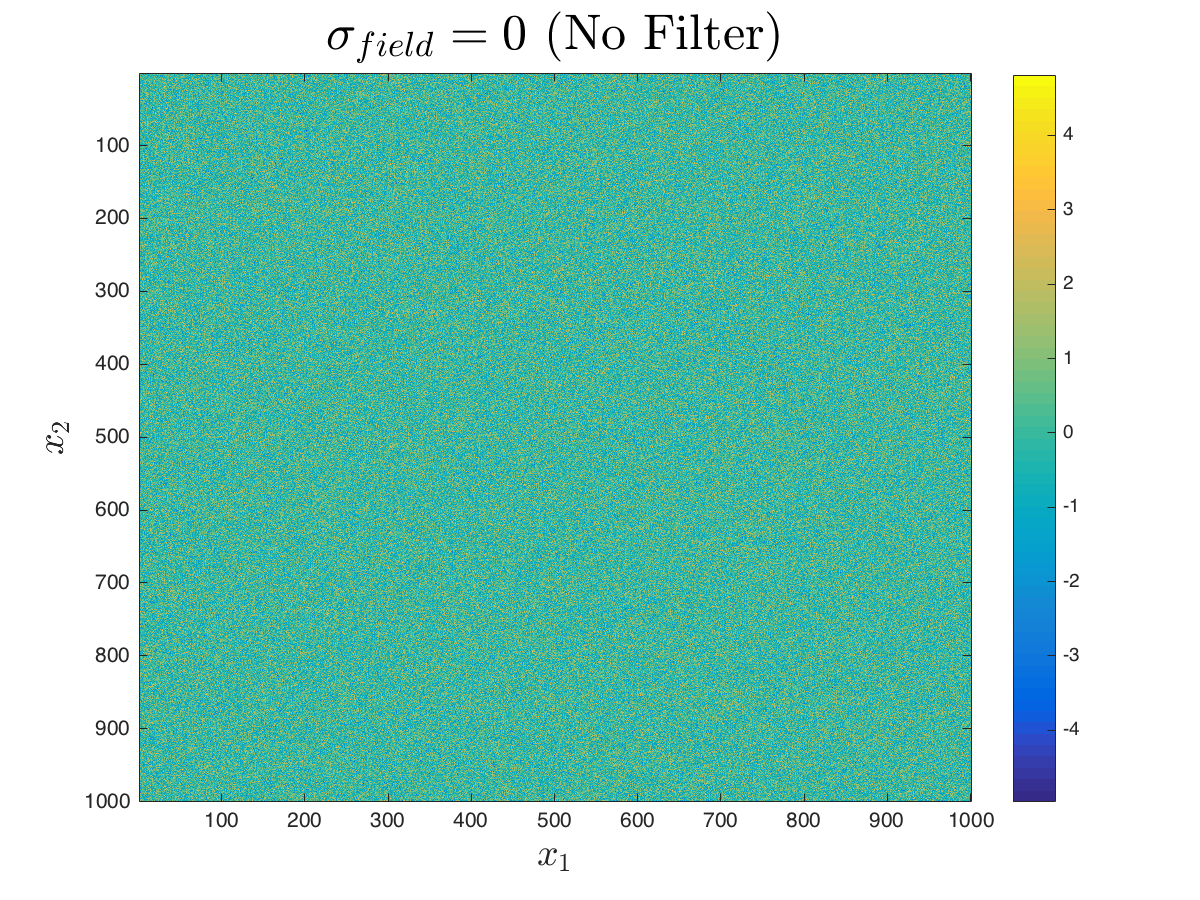
\includegraphics[width=\linewidth]{figures/autocorr_sigma_0.png}
        \captionsetup{skip=0.25\baselineskip,size=footnotesize}
        \ssp
        \caption{$\sigma_{field} = 0$. The field exhibits no spatial autocorrelation.}
    \end{subfigure}%
    ~
    \begin{subfigure}[t]{0.33333\textwidth}
        \centering
        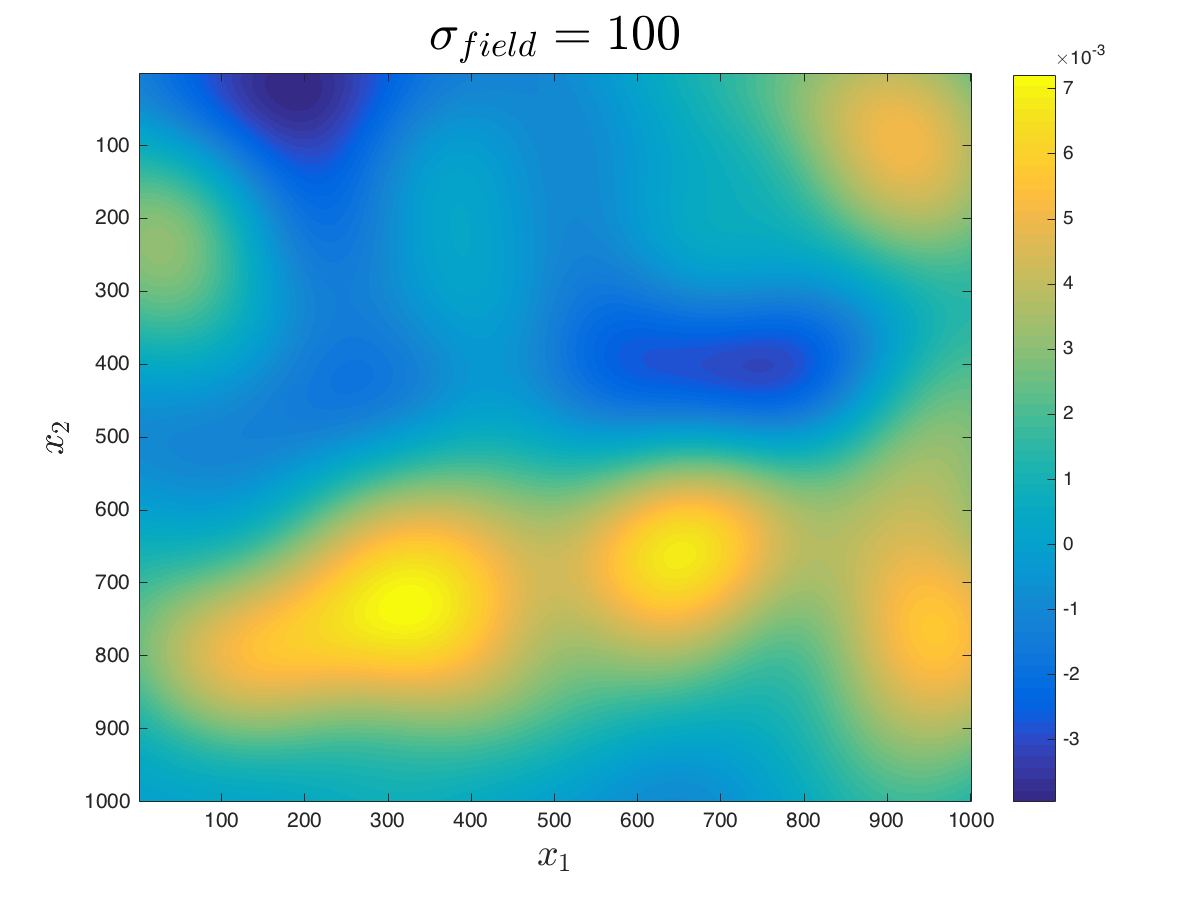
\includegraphics[width=\linewidth]{figures/autocorr_sigma_100.png}
        \captionsetup{skip=0.25\baselineskip,size=footnotesize}
        \ssp
        \caption{$\sigma_{field} = \frac{w}{10} = 100$. The field appears to exhibit some degree of spatial autocorrelation.}
    \end{subfigure}%
    ~ 
    \begin{subfigure}[t]{0.33333\textwidth}
        \centering
        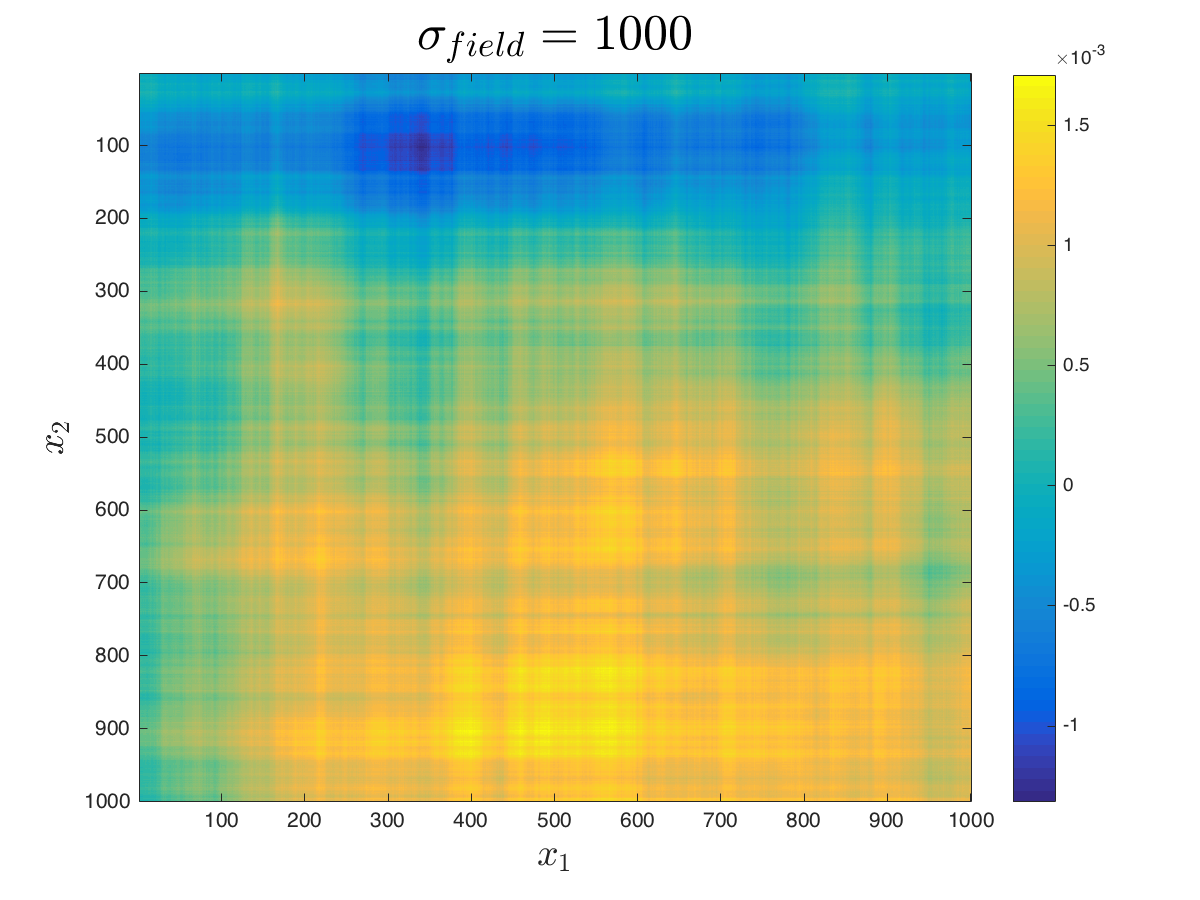
\includegraphics[width=\linewidth]{figures/autocorr_sigma_1000.png}
		\captionsetup{skip=0.25\baselineskip,size=footnotesize}
		\ssp
        \caption{$\sigma_{field} = w = 1000$. The field exhibits a high degree of spatial autocorrelation.}
    \end{subfigure}
    \ssp
    \caption{A field is generated using a random number generator with a zero mean normal distribution with variance $1$. Varying degrees of spatial autocorrelation are shown for different values of $\sigma_{field}$.}
\end{figure}

\section{Simulation Environment}
The simulation, once started, runs a single exploration method at a time starting with the same random number seed. A generated field is initially unknown to a vehicle object, but samples are collected as it passes along the field. The variances of Kriging predictions, the currently predicted field, and the path traversed are plotted along with the actual field being explored.

\begin{figure}[htb!]
    \centering
    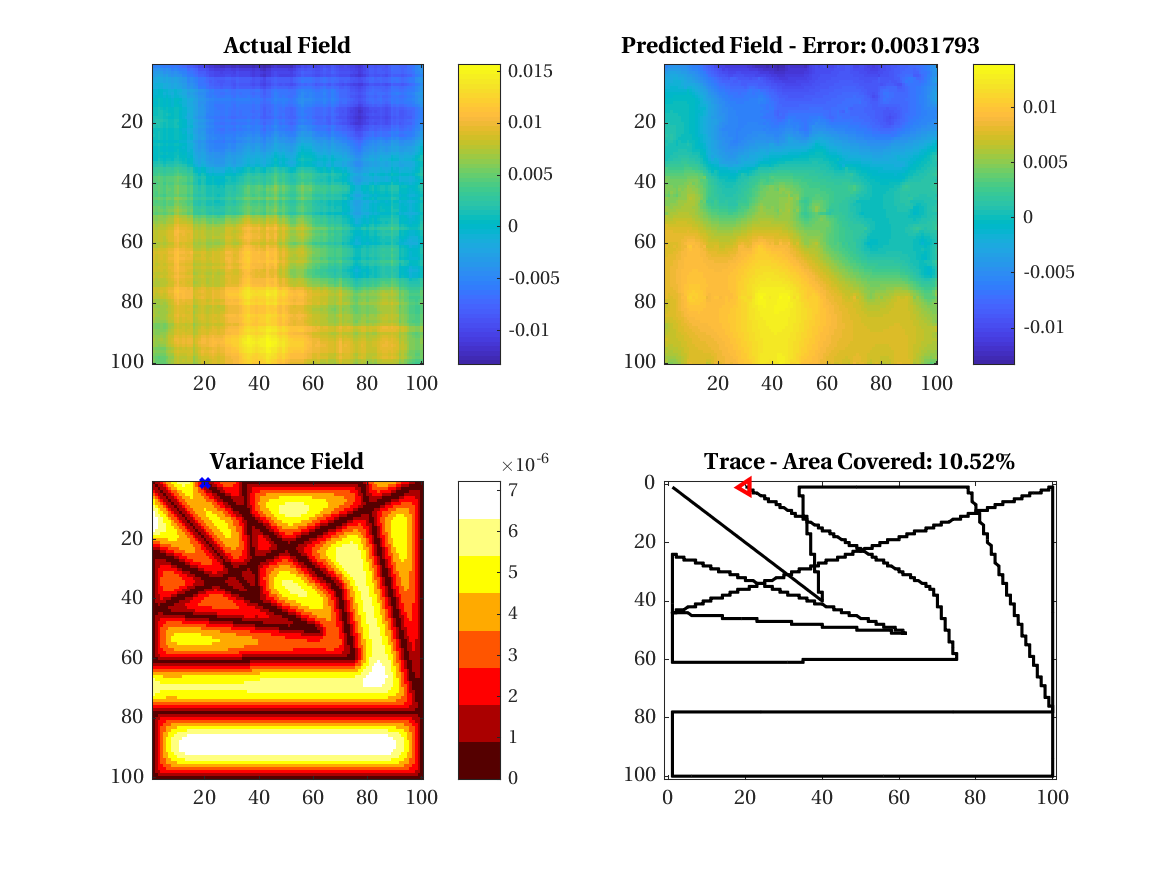
\includegraphics[width=0.8\linewidth]{figures/sim_figures/nhv_10p_100x100_sf_50_seed_2.png}
	\captionsetup{skip=0.25\baselineskip}
	\ssp
    \caption{Highest Variance Path Planning. The actual field (top left), predicted field (with error) (top right), variance field (bottom left), and traversed path (bottom right).}
\end{figure}

\begin{figure}[htb!]
    \centering
    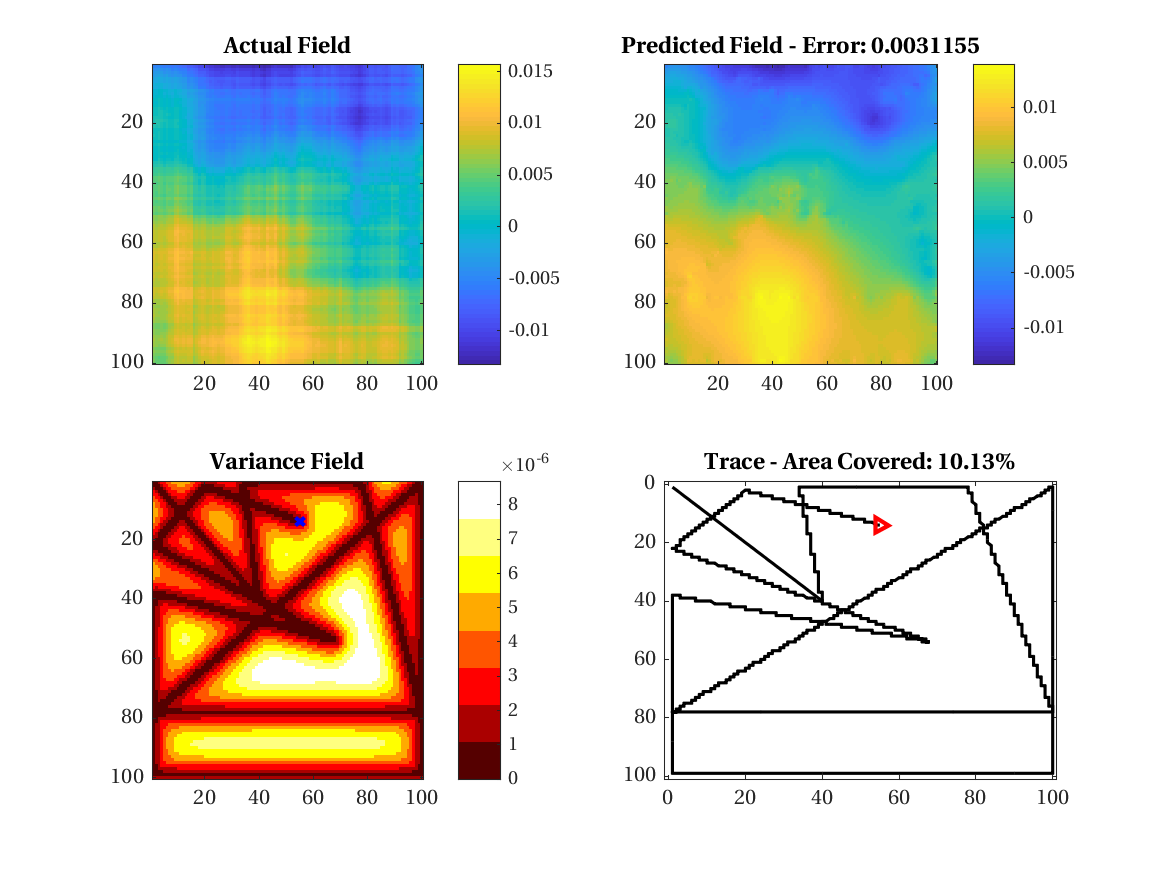
\includegraphics[width=0.8\linewidth]{figures/sim_figures/nnhv_10p_100x100_sf_50_seed_2}
    \captionsetup{skip=0.25\baselineskip}
    \ssp
    \caption{$N$ Highest Variance Path Planning ($N=5$). The actual field (top left), predicted field (with error) (top right), variance field (bottom left), and traversed path (bottom right).}
\end{figure}

\begin{figure}[htb!]
    \centering
    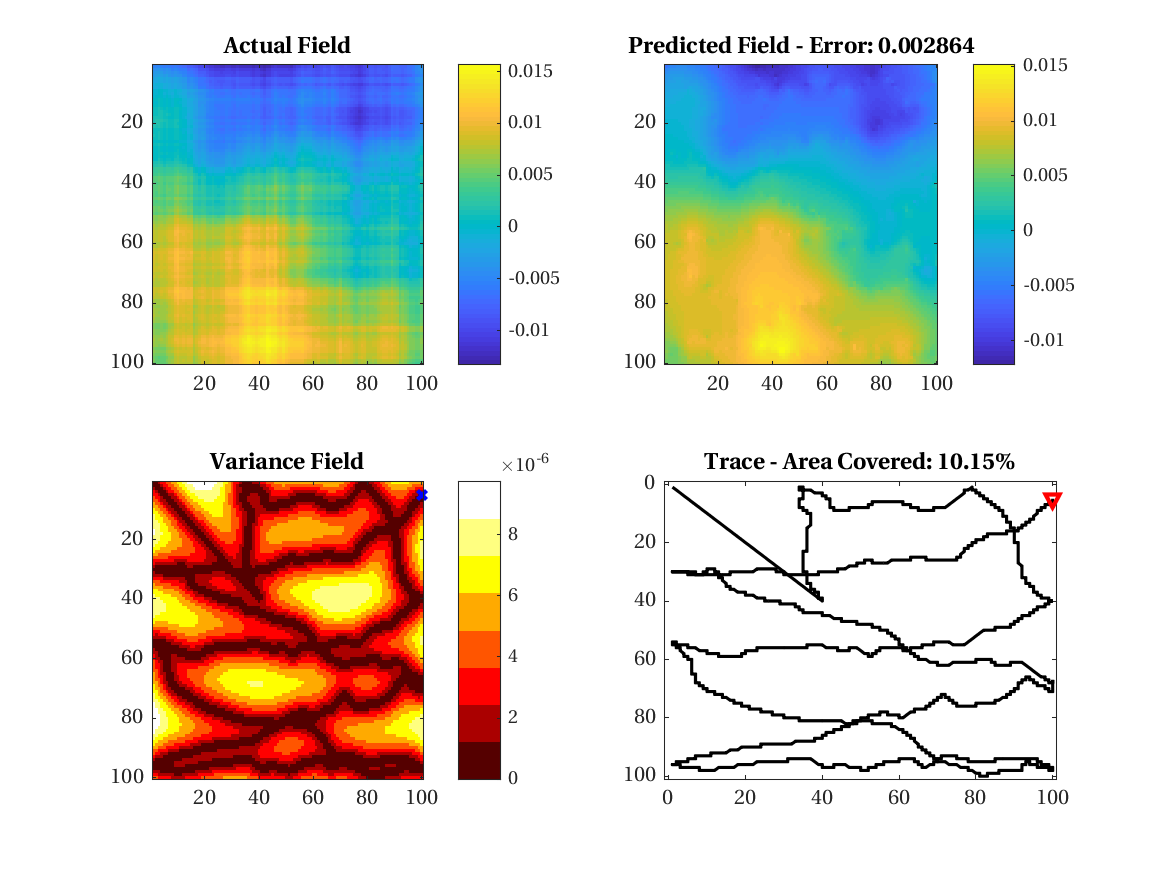
\includegraphics[width=0.8\linewidth]{figures/sim_figures/mc_10p_100x100_sf_50_seed_2}
    \captionsetup{skip=0.25\baselineskip}
    \ssp
    \caption{Monte Carlo Path Planning ($N=5$, $M_{mc}=5$). The actual field (top left), predicted field (with error) (top right), variance field (bottom left), and traversed path (bottom right).}
\end{figure}

\begin{figure}[htb!]
    \centering
    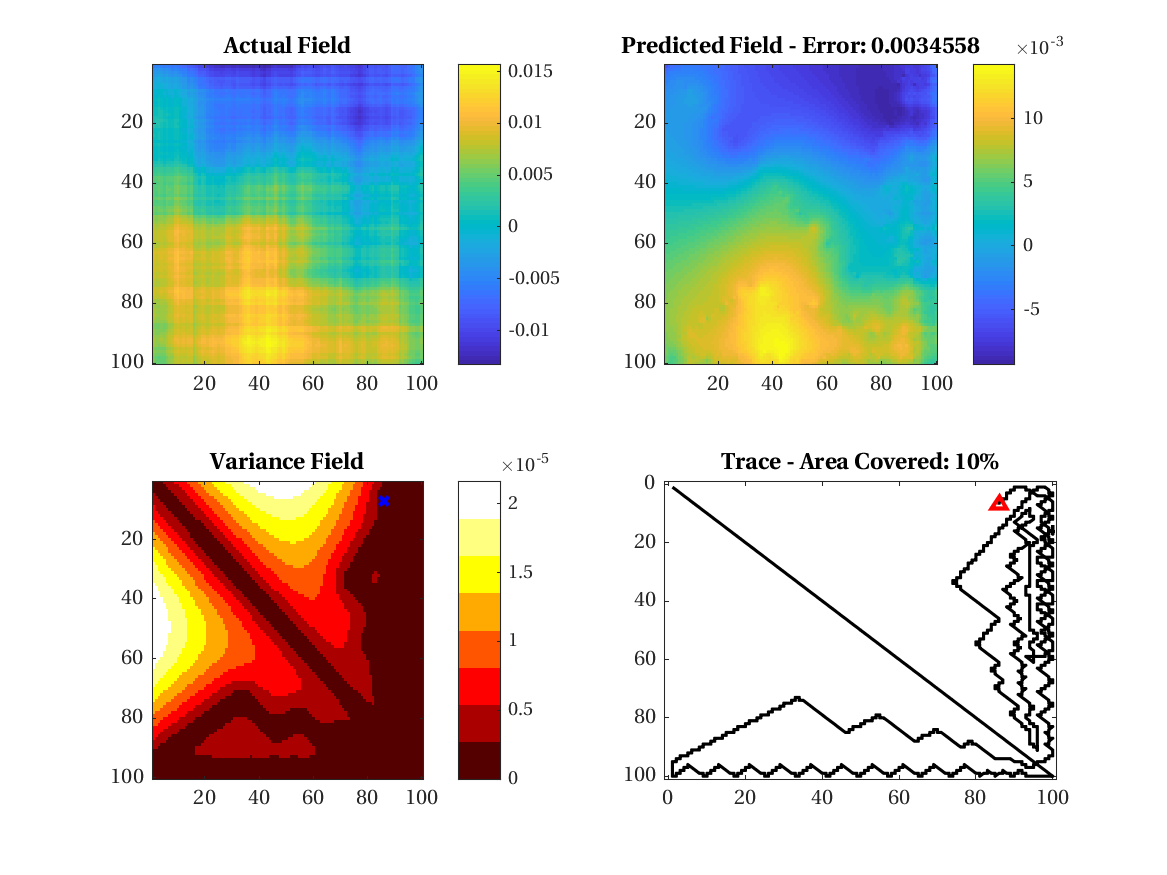
\includegraphics[width=0.8\linewidth]{figures/sim_figures/gradient_10p_100x100_sf_50_seed_2}
    \captionsetup{skip=0.25\baselineskip}
    \ssp
    \caption{Gradient Ascent Path Planner. The actual field (top left), predicted field (with error) (top right), variance field (bottom left), and traversed path (bottom right).}
\end{figure}

\begin{figure}[htb!]
    \centering
    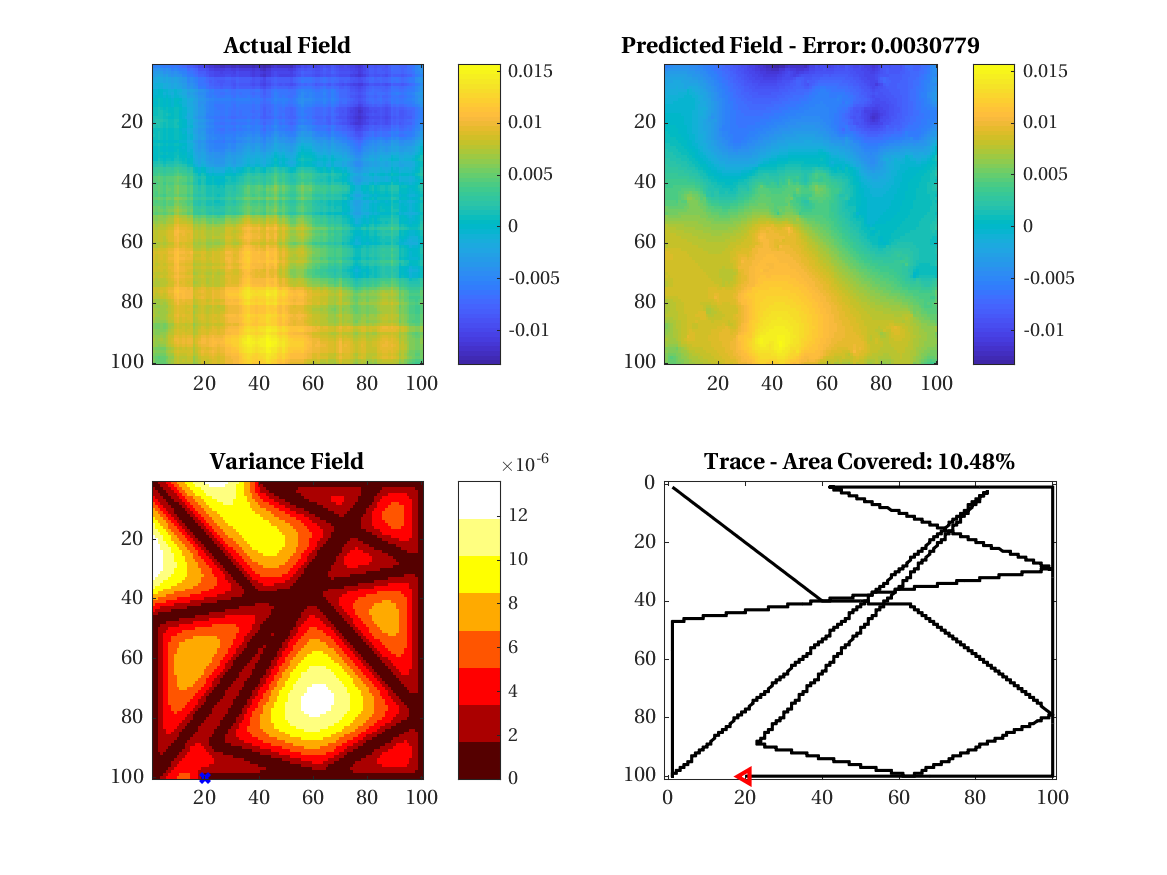
\includegraphics[width=0.8\linewidth]{figures/sim_figures/gr_10p_100x100_sf_50_seed_2}
    \captionsetup{skip=0.25\baselineskip}
    \ssp
    \caption{Range Gradient Ascent Path Planner. The actual field (top left), predicted field (with error) (top right), variance field (bottom left), and traversed path (bottom right).}
\end{figure}

\begin{figure}[htb!]
    \centering
    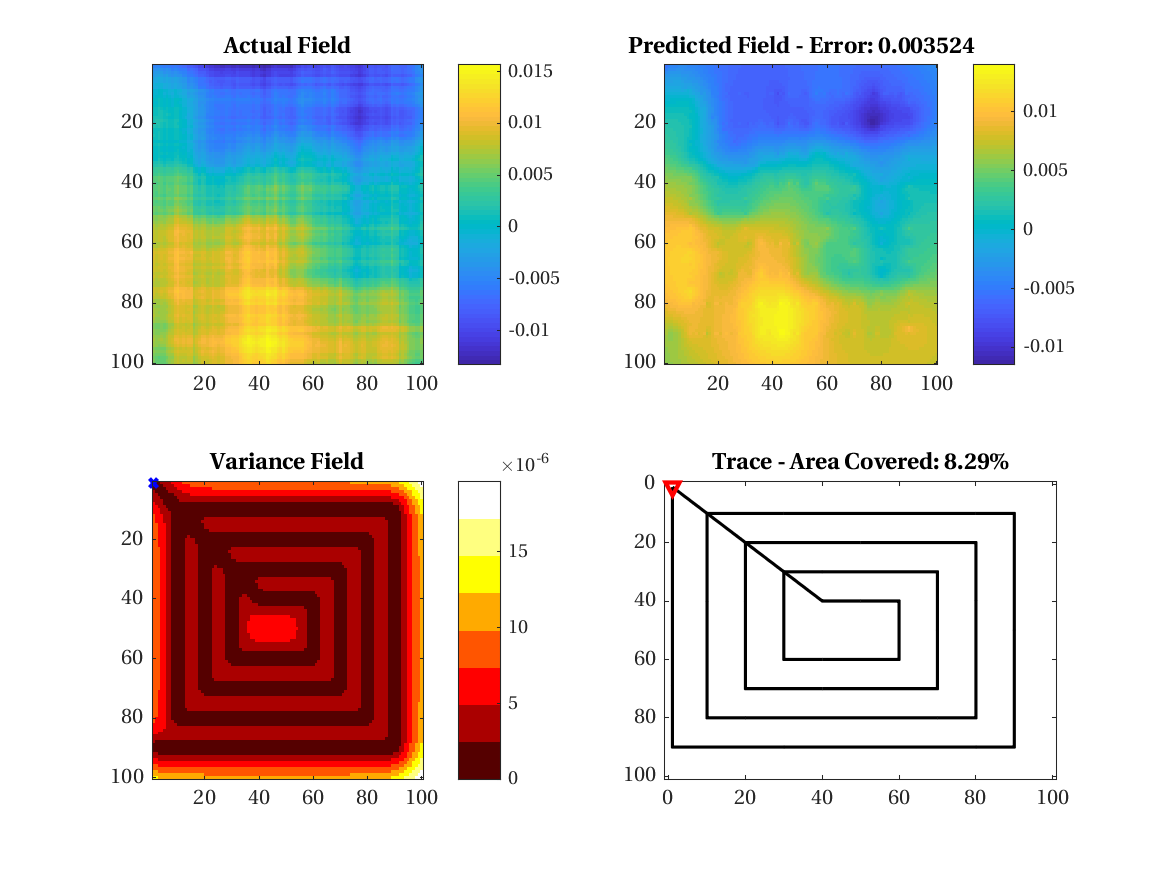
\includegraphics[width=0.8\linewidth]{figures/sim_figures/zz_10p_100x100_sf_50_seed_2}
    \captionsetup{skip=0.25\baselineskip}
    \ssp
    \caption{Zig-Zag Method. The actual field (top left), predicted field (with error) (top right), variance field (bottom left), and traversed path (bottom right).}
\end{figure}
